\documentclass[a4paper, itemph]{oblivoir}
\setmainhangulfont{NANUMMYEONGJO.TTF}[BoldFont={NANUMMYEONGJOEXTRABOLD.TTF}]
\usepackage[english]{babel}
\usepackage[utf8x]{inputenc}
\usepackage[T1]{fontenc}
%% Sets page size and margins
\usepackage[a4paper,top=3cm,bottom=2cm,left=3cm,right=3cm,marginparwidth=2cm]{geometry}

\usepackage{indentfirst}

%% Useful packages
\usepackage{amsfonts}
\usepackage{amsmath, mathtools}
\usepackage{graphicx}
\usepackage{subcaption}
\usepackage[colorinlistoftodos]{todonotes}
\usepackage{amssymb}
\usepackage{amsthm}
\usepackage{tikz}

%Extravaganza
\newtheorem{thm}{Theorem}[subsection]
\newtheorem{lem}{Lemma}[subsection]
\newtheorem{cor}{Corollary}[subsection]
\newcommand{\overbar}[1]{\mkern 1.5mu\overline{\mkern-1.5mu#1\mkern-1.5mu}\mkern 1.5mu}
\theoremstyle{definition}
\newtheorem{defn}{Definition}[subsection]
\newtheorem{rem}{Remark}[subsection]

\begin{document}
\title{기초전자회로 및 실험: Lab \#03}
\author{서울대학교 전기$\cdot$정보공학부 2018-12602 이준협}
\date{April 18, 2020}
\maketitle
\begin{figure}[htb]
    \centering
    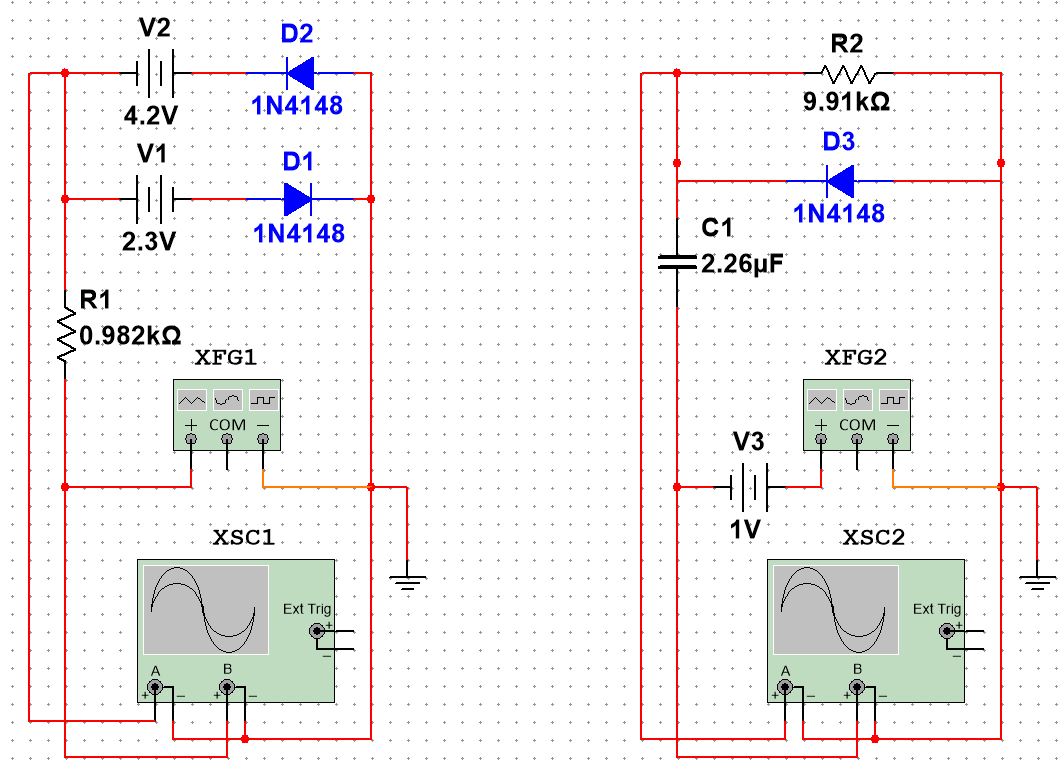
\includegraphics[width=0.5\linewidth]{lab3.PNG}
    \caption{Circuits as used in the experiments. Left: limiter($V_{in}=7.80$[$\mathrm{V_p}$]. 100Hz sinusoid). Right: clamping($V_{in}:$ 1kHz square wave with low: -5.001[V], high: 3.080[V]).}
\end{figure}

\section{Limiter Circuit}

\begin{table}[htb]
    \centering
    \begin{tabular}{c|c|c}
         &  High[V] & Low[V]\\
         \hline
         $V_{out}$& 3.011 & -5.00
    \end{tabular}
    \caption{Limited voltages in the limiting circuit.}
\end{table}
The circuit worked as designed, limiting the $\pm$7.80[V] input voltage at -5.00[V] and 3.011[V]. The turn on voltage of the two diodes were different; the diode limiting the voltage at 3.011[V] was turned on at 3.011-2.3=0.7[V], and the other diode was turned on at 5.00-4.2=0.8[V]. This indicates that more current was flowing through the diode when the voltage is limited at 5.00[V]. However, calculations show that this is not the case. When the output is -5.00[V], the current flowing through the resistor is maximum $(7.80-5.00)/0.982=2.85$[mA], and therefore the current flowing through D2(in figure 1) is $2.85$[mA], since D1 is reverse biased and therefore cannot carry much current. When the output is 3.011[V], the current flowing through D1 is $(7.80-3.011)/0.982=4.88$[mA]. 

The measurement of the difference of voltages by the oscilloscope and the measurement of the resistance by the multimeter are accurate up to at least $10^{-3}$. Also, current couldn't be drawn from the oscilloscope since the probe input impedance is $10$[M$\Omega$], which is $10^5$ times the small-signal resistance of the diode($V_T/I_D$ is in the $10\Omega$ range), therefore the diode must dominate the current by 99.99\%. Thus the forward bias on D1 must be higher than D2 as indicated by the currents. One explanation for this measurement is that the measured $V_{out}$ is shifted down by a DC bias. Since the probe ground wire measuring $V_{out}$ is further from the ground tab on the breadboard than the ground wire measuring $V_{in}$, the wire resistance pulls down $V_{out}$.
\section{Clamping Circuit}
\begin{table}[htb]
    \centering
    \begin{tabular}{c|c|c|c|c}
         & Forward bias, min[V] & Forward bias, max[V] & Reverse bias, max[V] & Reverse bias, min[V]\\
         \hline
         $V_{out}$& -0.7203 & -0.600 & 7.440 & 7.20
    \end{tabular}
    \caption{Output voltage of clamping circuit, measured in average acquisition mode.}
\end{table}
The voltage was pulled up to $7.440=8-0.560\approx 8-V_{d,on}$, and decayed 0.24[V], which is less than 0.3[V]. Thus, the circuit works as expected. However, there are some discrepancies with theory.

The input voltage was measured to transition from -5.001[V] to 3.080[V]. Since the voltage across a capacitor is continuous, the output voltage must also be pulled up and pulled down by $3.080+5.001=8.081$[V] every half period. However, the output is pulled up by $7.440+0.600=8.040$[V] and pulled down by $7.20+0.7203=7.92$[V]. Therefore, we need to consider the parasitic impedance connected in series with the capacitor. When the input changes from low to high, the diode is reverse biased, and the current flows to ground through the resistor, therefore the voltage is pulled up less than expected due to the voltage drop across the series impedance. When the input changes from high to low, the diode is forward biased, therefore the current flows from ground to the capacitor, so the series resistor pulls up the output voltage. This explains why the voltage difference at each half period was measured to be less than expected. 

The voltage decay due to the $RC$ circuit when the diode is in the forward bias region is $0.120$[V], and the voltage decay when the diode is in the reverse bias region is $0.24$[V]. Assuming that the current that supplied charges to the capacitor is constant during the short 0.5[ms] half-period, we can say that the current that was supplied to the capacitor from the ground(diode turned on) was $C\Delta V/\Delta t=2.26\times 0.120/0.5=0.542$[mA]. Likewise, the current that was supplied from the capacitor to the ground was $2.26\times 0.24/0.5=1.08$[mA]. The 0.542[mA] was supplied from the 0.982[k$\Omega$] resistor, which had a voltage of 720.3[mV] across it, and the diode. Since the resistor supplies a current of $0.7203/9.91=0.0727$[mA], the diode must supply an current of $0.469$[mA] with an average bias of $660$[mV], which fits with measurements made in lab 1. Meanwhile, the 1.08[mA] must be carried almost entirely by the resistor, since the current through the diode in reverse bias is in the nA range. However, the current flowing through the resistor is $7.440/9.91=0.751$[mA]. Although $1.08-0.751=0.329<0.469$(the current supplied in forward bias), $0.329$[mA] is not a current able to be supplied by a diode in the reverse bias region according to theory. This result is mainly due to nonideality of the diode; the reverse recovery time in the 1N4148 datasheet was measured when the reverse current is 1[mA][1], so it indicates that in switching conditions, the reverse current may hit the 1[mA] range.
\section{Limitations in the Limiting Circuit}

Let the maximum limit be $V_1$, the minimum limit be $V_2$. The DC bias connected to each diode must pull up $V_1-V_{d,on}$ and $V_{d,on}+V_2$ relative to ground. The maximum reverse voltage on each diode is $V_1-V_2+V_{d,on}$, and the maximum forward current is $\dfrac{\max(V_p-V_1, V_p+V_2)}{R}$. Since in each half cycle only one diode is turned on, one may use the maximum repetitive peak forward current and the maximum repetitive peak reverse voltage. The maximum reverse voltage is 75[V], so $V_1-V_2$ cannot be any higher than $75-V_{d,on}$. The maximum repetitive peak forward current of the 1N4148 is 450[mA], therefore for oscillating signals with peak voltage $V_p$[V], the maximum current through the resistor in the case of this experiment, $(V_p-3)/0.982$[mA] must be no greater than 450[mA]. Then the maximum peak voltage is 444.9[V][1].
\section{Discussion}
The qualitative properties of the designed circuits were as expected, with a near-constant voltage in the 500 to 800[mV] range maintained on the diode and current being limited in the reverse bias region compared to the forward bias region. However, due to the nonidealities in the diode and due to series/parallel parasitic impedance, more current may flow through the circuit as a result. When simulated by MultiSim as in Figure 1, the clamping circuit displayed a peak of 7.465[V] which decayed to 7.302[V] and a minimum of -692.156[mV] which decayed to -534.440[mV]. Thus, the reverse bias current is still measured to be in the 0.2[mA] region, and this again confirms the nonideality of the diode.

The theoretical reason for this nonideality is explained in [2], and it explains that the dynamic junction capacitance in the reverse bias region creates charge flow when the voltage oscillates across the diode. This can be modelled as a series capacitance connected to the ideal diode, and in the reverse region the diode can be thus replaced by the small capacitor, since an ideal diode can be viewed as an open node in reverse bias conditions. Thus, in real design problems the frequency must also be considered when designing diode circuits.

\begin{thebibliography}{}

\bibitem{1} \textit{1N4148; 1N4448
High-speed Diodes Product Specification}, Philips Semiconductors, 1999 May 25. Accessed on: April 17, 2020. [Online]. Available: \texttt{https://global.oup.com/us/companion.\\websites/fdscontent/uscompanion/us/pdf/microcircuits/students/diode/1n4148-philip.pdf}
\bibitem{2} F. Clifton, \textit{Microelectronic Devices and Circuits}, 2006, pp. 161-162. Accessed on: April 17, 2020. [Online]. Available: \texttt{http://dspace.mit.edu/handle/1721.1/34219}

\end{thebibliography}

\end{document}
